\documentclass[a4paper,12pt]{article}
\usepackage[utf8]{inputenc}
\usepackage{geometry}
\geometry{a4paper, margin=2.5cm}
\usepackage{graphicx}
\usepackage{amsmath, amssymb}
\usepackage{biblatex}
\usepackage{hyperref}
\usepackage{tikz}
\usetikzlibrary{positioning}

\addbibresource{references.bib}

\title{Förderantrag für ein SOTL-Projekt: Problembasiertes Lernen in der KI-Lehre}
\author{Alexander Rachmann}
\date{\today}

\begin{document}

\maketitle

\section{Ausgangslage}

Am Fachbereich Wirtschaftsingenieurwesen verflechten wir (Prof. Rachmann und Prof. Poschmann) in das Curriculum derzeit an mehreren Stelle Kompetenzen in der Programmierung und der Nutzung von Künstlicher Intelligenz. Dafür wählen wir derzeit oft einen projektbasierten Ansatz, in dem wir Studierenden Aufgaben übertragen und sie in der Erledigung dieser Aufgaben coachen. 

Als Beispiel (Lehveranstaltung "KI-Anwendungen im betriebliche Umfeld" im Wintersemester 2024/25): Wir übertrugen einer 4-Personen-Gruppe die Aufgabe einen Chatbot zu entwickeln, vermittelten Grundlagen zur Programmierung dieser Chatbots. Zu regelmäßigen Gesprächsterminen luden wir die Studierenden ein, sich Feedback einzuholen. Diese Gesprächstermine ließen wir bewusst optional, damit die Studierenden sich eigeninitiativ entwickeln und eigene Fragen erarbeitenkönnen.

Diese Vorgehen war gut gemeint. Aber es traten die folgenden Nachteile auf: Die Studierenden nehmen zu Anfang des Semesters die optionalen Termine wenig wahr und kommen (aus unserer Sicht) zu langsam voran. Den Studierenden aktivieren sich zum Ende des Semesters. Dadurch sind die Studierenden am Ende des Semesters einerseits gestresst, andererseits bleibt der Lerneffekt für sie (vermutlich) minimal.

\section{Forschungsmotivation}

Wir möchten die Studierenden in die Lage versetzen im Semesterverlauf regelmäßiger an ihrer Aufgabe zu arbeiten, dadurch in weniger (negativ empfundene) Stresssituationen zu kommen und dadurch mehr zu lernen.

Wir denken, dass eine intensivere, nicht-optionale Betreuung der Studierenden zu einer besseren Lernsituation führen könnte. Gleichzeitig möchten wir die Studierenden aber in einer Situation halten, in der sie eigeninitiativ und -verantwortlich agieren.



\section{Forschungsansatz}

\subsection{Ansätze zur Integration von agiler Arbeit und PBL}
In mehreren Forschungsarbeiten zur Informatikdidaktik wurden Ansätze beschrieben, die ein ähnliches Zielbild verfolgen. Dabei werden oftmals typische Projektmanagement-Methoden für die Softwareentwicklung mit didaktischen Konzepten kombiniert: Scrum und Project Based Learning \cite{fernandes2021improving}, Scrum und Challenge based Learning \cite{santos2015combining} oder Scrum und Problem based Learning \cite{da2022scrum}. Insbesondere \cite{da2022scrum} zeigt eine niedrigschwellige Verbindung der beiden Ansätze, welches für unsere Situation anpassbar erscheint. Auch \cite{meissner2015brauchen} und \cite{kenneweg2025problem} zeigen Ansätze, wie problem based Learning in iterativen Prozessen gewinnbringend eingesetzt werden kann.


%\section{Hintergrund und Relevanz}
%Problembasiertes Lernen (PBL) ist eine bewährte Methode zur Förderung kritischen Denkens und eigenständiger Problemlösungsfähigkeiten \cite{barrows1986framework, meissner2015brauchen}. Insbesondere im Bereich der KI, in dem Studierende oft mit komplexen und offenen Fragestellungen konfrontiert sind, bietet PBL einen vielversprechenden Ansatz \cite{collins1989cognitive, kenneweg2025problem}. Frühere Studien zeigen, dass PBL zu besseren Lernergebnissen führen kann, indem es die aktive Auseinandersetzung mit Lerninhalten fördert \cite{dolmans2015problem}.



\subsection{Didaktische Planung der Veranstaltungen}

Abbildung \ref{fig:scrum_pbl} zeigt, wie Scrum und PBL in das Lehrkonzept integriert werden können. Hierbei unterscheiden wir zwischen der Scrum-Sicht, der problem-based learning-Sicht und der SOTL-Sicht.

Von Scrum wird eine vereinfachte Form übernommen: Es gibt einen Product Backlog, aus dem von den Studierenden ein Sprint Backlog generiert wird. Im PBL-Schritt 2 wird die erste Anpassung bei PBL-sichtbar: Im Sprint Backlog befinden sich nun Teil-Probleme. Diese Teilprobleme bilden zusammen das Problem im Sinne des problem-based learning. Hinter dieser Aufteilung steckt die Annahme, dass das Problem zu komplex ist, als in einem Sprint gelöst zu werden. Eine zweite Anpassung findet in PBL-Schritt 5 statt: Es werden "Aufgaben" ergänzt; ggf. gibt es im Semester Tätigkeiten, die keinen direkt Lerneffekt erzielern, aber doch gemacht werden müssen um einen anderen Lerneffekt zu erzielen.

Die von \cite{kenneweg2025problem} "Selbststudium" benannte Phase wird in der Abbildung als "Lösungsorientierte Arbeit" benannt. Hierhinter verbirgt sich auch Arbeit einer einzelnen Person und Selbstudium, aber letztlich auch Teamarbeit während des Sprints.

\cite{kenneweg2025problem} schlägt einen optionalen achten PBL-Schritt vor, der in der zweiten Gruppenphase verortet ist. In der Scrum-Sicht ist dies als Review und Retro etabliert. Hierbei findet auch die Messung in der SOTL-Sicht statt.


\begin{figure}[ht]
    \centering
    \includegraphics[width=0.6\textwidth]{images/scrumundpblundsotl.png}
    \caption{Integration von Scrum und PBL im Lehrkonzept, in Anlehnung an \cite{da2022scrum} und \cite{kenneweg2025problem}}
    \label{fig:scrum_pbl}
\end{figure}

\clearpage

In einem Semester werden vier dreiwöchige Sprints geplant, siehe Abbildung \ref{fig:semester}. Dementsprechend werden vier Messungen in der SOTL-Sicht vorgenommen. Die Sprints werden mit einer Einleitung und einem Abschluss versehen. In der Einleitung wird den Studierenden die Semesterorganisation vorgestellt, Gruppen gebildet, Prüfungsfragen gehlärt 


\begin{figure}[ht]
    \centering
    \includegraphics[width=1\textwidth]{images/semester.png}
    \caption{Vier Iterationen und Messungen in der Semestersicht}
    \label{fig:semester}
\end{figure}



\section{Forschungsansatz}
\subsection{Forschungshypothese}
Die Forschungshypothese lautet: Durch eine Integration von Scrum und PBL in das Lehrkonzept wächst die Kompetenz der Studierenden.

\begin{figure}[ht]
\begin{center}
    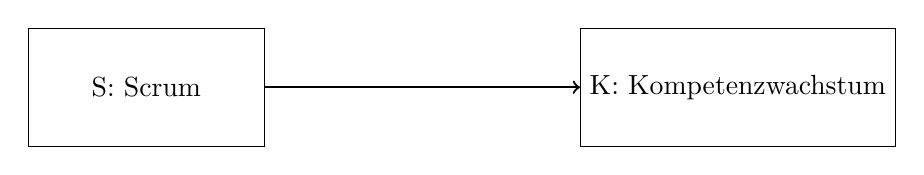
\begin{tikzpicture}
        \node[draw, rectangle, minimum width=3cm, minimum height=1.5cm] (A) {S: Scrum};
        \node[draw, rectangle, minimum width=3cm, minimum height=1.5cm, right=of A, xshift=3cm] (B) {K: Kompetenzwachstum};
        \draw[->, thick] (A) -- (B);
    \end{tikzpicture}
    \caption{Schema der Forschungshypothese}
\end{center}
\end{figure}

\subsection{Operationalisierung}
Die Operationalisierung der unabhängigen Variable S wird durch die Nummer der Iteration (\textbf{I}) gemessen: Es ist davon auszugehen, dass in der ersten Iteration die Studierenden noch wenig Kompetenz besitzen, in der zweiten Iteration mehr und in der vierten Iteration eine hohe Kompetenz aufgebaut haben.

Dies gilt sowohl für Studierende, die sich schon mit Scrum auskennen, als auch für Studierende, die sich noch nicht mit Scrum auskennen.

Die abhängige Variable K wird dreifach operationalisiert:
\begin{enumerate}
    \item Wachstum der technischen Kompetenz (\textbf{TK}): die Studierenden evaluieren selbst, ob ihre Kompetenzen in Softwareentwicklung gewachsen sind. Hierzu werden den Studierenden standardierte Fragen gestellt.
    \item Wachstum der methodischen Kompetenz (\textbf{MK}): die Studierenden evaluieren selbst, ob ihre methodischen Problemlösekompetenz (Anwendung von PBL und Scrum) gewachsen ist. Hierzu werden den Studierenden standardisierte Fragen gestellt.
    \item Artefaktbewertung (\textbf{AB}): Zum Ende einer Iteration wird das entwickelte Artefakt (typischerweise Software) vom Dozeierenden bewertet. Dies dient als objektivierte Kontrollmessung zu den subjektiven Befragungen der Studierenden. 
    
    Diese Bewertung ist nicht notenrelevant, sondern dient nur der Forschung.
\end{enumerate}

Es ist zu erwarten, dass in den späteren Iterationen tendenziell höhere Werte von TK, MK und AB erreicht werden. (Wenn "hoch" bedeutet, dass die Komptenz gewachsen ist.)

\begin{figure}[h]
\begin{center}
    \begin{tikzpicture}
        \node[draw, rectangle, minimum width=3cm, minimum height=1.5cm] (I) { I};
        \node[draw, rectangle, minimum width=3cm, minimum height=1.5cm, right=of I, xshift=3cm, yshift=-2cm] (TK) {TK};
        \node[draw, rectangle, minimum width=3cm, minimum height=1.5cm, right=of I, xshift=3cm] (MK) {MK};
        \node[draw, rectangle, minimum width=3cm, minimum height=1.5cm, right=of I, xshift=3cm, yshift=2cm] (AB) {AB};
        \draw[->, thick] (I) -- (TK);
        \draw[->, thick] (I) -- (MK);
        \draw[->, thick] (I) -- (AB);
    \end{tikzpicture}
    \caption{Schema der Operationalisierung}
\end{center}
\end{figure}

\subsection{Zeitplan}
\begin{tabular}{|l|l|}
    \hline
    Zeitraum & Aktivität \\
    \hline
    Mai, Juni, Juli & Ausarbeitung der konkreten Fragen zu Kompetenzmessung \\
    Wintersemester & Durchführung der Lehrveranstaltungen, Datenerhebung \\
    Februar, März, April & Auswertung und Publikation \\
    \hline
\end{tabular}








\section{Literatur}
\printbibliography

\end{document}
